\documentclass[11pt, a4paper]{article}
\usepackage[utf8]{inputenc}
\usepackage[spanish]{babel}
\usepackage{amsmath, amssymb, amsfonts}
\usepackage{graphicx}
\usepackage{geometry}
\geometry{left=2.5cm, right=2.5cm, top=2.5cm, bottom=2.5cm}
\usepackage{tikz}
\usepackage{bm}
\usepackage[hidelinks]{hyperref}
\graphicspath{{figs/}{../figs/}}


\title{\vspace{-1.5cm}\textbf{Resolución de Ecuaciones Diferenciales Ordinarias}\\ \large Métodos Matemáticos I --- Hoja 6}
\author{\textbf{César Endris Acosta}}

\date{10 de noviembre de 2026}
\begin{document}

\maketitle
\vspace{-0.2cm}

\begin{center}
\fbox{\parbox{0.93\linewidth}{\small
\textbf{Versión interactiva.} Todos los problemas de esta hoja se pueden visualizar e interactuar con sus gráficas
(constantes con deslizadores, curva elegida, campos de direcciones, etc.) en la página web
(pestaña ``Hoja 6''):\\[2pt]
\centerline{\url{https://endris10.github.io/Mathematical_Methods_1/}}\vspace{2pt}
Se utilizó IA (Claude, de Anthropic) \textbf{únicamente para programar la página web};
la resolución de las ecuaciones diferenciales es propia.}}
\end{center}

\noindent\textbf{1. Para cada una de las siguientes EDOs, localizad y clasificad sus puntos singulares.} \\
Un punto singular $x_0$ es \emph{regular} si $(x-x_0)P(x)$ y $(x-x_0)^2Q(x)$ son analíticas en $x_0$, e \emph{irregular} en caso contrario.

\begin{itemize}
\item \textbf{(a) $\bm{x^3(x-1)y''-2(x-1)y'+3xy=0}$:} \\
$P(x)=\dfrac{-2(x-1)}{x^3(x-1)}=-\dfrac{2}{x^3}, \qquad Q(x)=\dfrac{3x}{x^3(x-1)}=\dfrac{3}{x^2(x-1)}$. Puntos singulares: $x=0$ y $x=1$.
\begin{itemize}
\item $x=0$: $xP(x)=-\dfrac{2}{x^2}$ no es analítica en $0$ $\implies$ \textbf{irregular}.
\item $x=1$: $(x-1)P(x)=-\dfrac{2(x-1)}{x^3}$ y $(x-1)^2Q(x)=\dfrac{3(x-1)}{x^2}$ son analíticas en $1$ $\implies$ \textbf{regular}.
\end{itemize}

\item \textbf{(b) $\bm{x^2(x^2-1)^2y''-x(1-x)y'+2y=0}$:} \\
Como $-x(1-x)=x(x-1)$ y $x^2(x^2-1)^2=x^2(x-1)^2(x+1)^2$:
\[
P(x)=\frac{1}{x(x-1)(x+1)^2}, \qquad Q(x)=\frac{2}{x^2(x-1)^2(x+1)^2}
\]
Puntos singulares: $x=0,\ 1,\ -1$.
\begin{itemize}
\item $x=0$: $xP=\dfrac{1}{(x-1)(x+1)^2}$ y $x^2Q=\dfrac{2}{(x^2-1)^2}$ analíticas $\implies$ \textbf{regular}.
\item $x=1$: $(x-1)P=\dfrac{1}{x(x+1)^2}$ y $(x-1)^2Q=\dfrac{2}{x^2(x+1)^2}$ analíticas $\implies$ \textbf{regular}.
\item $x=-1$: $(x+1)P=\dfrac{1}{x(x-1)(x+1)}$ tiene un polo en $-1$ $\implies$ \textbf{irregular}.
\end{itemize}

\item \textbf{(c) $\bm{x^2y''+(2-x)y'=0}$:} \\
$P(x)=\dfrac{2-x}{x^2}, \quad Q(x)=0$. Único punto singular: $x=0$.
\begin{itemize}
\item $x=0$: $xP=\dfrac{2-x}{x}$ no es analítica en $0$ $\implies$ \textbf{irregular}.
\end{itemize}

\item \textbf{(d) $\bm{(3x+1)xy''-(x+1)y'+2y=0}$:} \\
$P(x)=-\dfrac{x+1}{x(3x+1)}, \quad Q(x)=\dfrac{2}{x(3x+1)}$. Puntos singulares: $x=0$ y $x=-\tfrac13$.
\begin{itemize}
\item $x=0$: $xP=-\dfrac{x+1}{3x+1}$ y $x^2Q=\dfrac{2x}{3x+1}$ analíticas $\implies$ \textbf{regular}.
\item $x=-\tfrac13$: $(x+\tfrac13)P=-\dfrac{x+1}{3x}$ y $(x+\tfrac13)^2Q=\dfrac{2(3x+1)}{9x}$ analíticas $\implies$ \textbf{regular}.
\end{itemize}
\end{itemize}


\noindent\textbf{2. Determinad la naturaleza del punto $\bm{x=0}$ para cada una de las siguientes EDOs.} \\
Usamos $\sin x = x - \dfrac{x^3}{6}+\dots$ y $P=0$ en todos los casos.
\begin{itemize}
\item \textbf{(a) $\bm{y''+(\sin x)y=0}$:} $Q=\sin x$ es analítica en $0$ $\implies$ \textbf{punto ordinario}.
\item \textbf{(b) $\bm{xy''+(\sin x)y=0}$:} $Q=\dfrac{\sin x}{x}=1-\dfrac{x^2}{6}+\dots$ es analítica en $0$ (singularidad evitable) $\implies$ \textbf{punto ordinario}.
\item \textbf{(c) $\bm{x^2y''+(\sin x)y=0}$:} $Q=\dfrac{\sin x}{x^2}$ , $x^2Q=\sin x$ es analítica $\implies$ \textbf{punto singular regular} (ecuación indicial $m(m-1)=0$).
\item \textbf{(d) $\bm{x^3y''+(\sin x)y=0}$:} $x^2Q=\dfrac{\sin x}{x}$ es analítica ($\to1$) $\implies$ \textbf{punto singular regular}
\item \textbf{(e) $\bm{x^4y''+(\sin x)y=0}$:} $x^2Q=\dfrac{\sin x}{x^2}\sim\dfrac1x$ no es analítica $\implies$ \textbf{punto singular irregular}.
\end{itemize}

\noindent\textbf{3. Verificad que el origen es un punto singular regular y calculad dos soluciones en forma de series de Frobenius.} \\
\textbf{Para $x>0$}  Proponemos $y=\sum_{n=0}^\infty a_nx^{n+m}$ con $a_0\neq0$. En cada término de la EDO sustituimos directamente
\[
y\to\sum_{n=0}^\infty a_nx^{n+m},\qquad y'\to\sum_{n=0}^\infty (n+m)a_nx^{n+m-1},\qquad y''\to\sum_{n=0}^\infty (n+m)(n+m-1)a_nx^{n+m-2},
\]
El término $n=0$ da la \emph{ecuación indicial} y los términos $n\geq1$ dan la \emph{fórmula de recurrencia}. \\
\textbf{Caso $\bm{x<0}$.} Se hace $z=-x>0$ y $y(x)=u(z)$, de modo que $y'=-u'$ e $y''=u''$ (derivadas respecto de $z$). Se resuelve la EDO transformada con $u=\sum_{n=0}^\infty b_nz^{n+m}$ y se deshace el cambio.

\medskip
\noindent\textbf{(a) $\bm{2xy''+(3-x)y'-y=0}$:} \\
$xP=\dfrac{3-x}{2}$ y $x^2Q=-\dfrac{x}{2}$ son analíticas en $0$ $\implies$ $x=0$ es singular regular.

\vspace{0.2cm}\noindent\textbf{ $\bm{x>0}$.} Sustituyendo cada término ya desarrollado:
\begin{align*}
2xy'' &\to \sum_{n=0}^\infty 2(n+m)(n+m-1)a_nx^{n+m-1} \\
3y' &\to \sum_{n=0}^\infty 3(n+m)a_nx^{n+m-1} \\
-xy' &\to -\sum_{n=0}^\infty (n+m)a_nx^{n+m} \\
-y &\to -\sum_{n=0}^\infty a_nx^{n+m}
\end{align*}
Desplazamos $n\to n-1$ en los dos últimos (ahora con exponente $x^{n+m-1}$ y suma desde $n=1$):
\begin{align*}
-xy' &\to -\sum_{n=1}^\infty (n+m-1)a_{n-1}x^{n+m-1}, \qquad -y \to -\sum_{n=1}^\infty a_{n-1}x^{n+m-1}
\end{align*}
Agrupando en $x^{n+m-1}$ (usando $2(n+m)(n+m-1)+3(n+m)=(n+m)\big(2(n+m)+1\big)$):
\[
m(2m+1)a_0x^{m-1}+\sum_{n=1}^\infty\Big[(n+m)\big(2(n+m)+1\big)a_n-(n+m)a_{n-1}\Big]x^{n+m-1}=0
\]

\smallskip\noindent $n=0$ (ecuación indicial): $m(2m+1)=0 \implies m_1=0,\quad m_2=-\tfrac12$.

\smallskip\noindent $n\geq1$ (recurrencia): $(n+m)\big(2(n+m)+1\big)a_n=(n+m)a_{n-1} \implies a_n=\dfrac{a_{n-1}}{2(n+m)+1}$.

\smallskip\noindent $m=0$: $a_n=\dfrac{a_{n-1}}{2n+1} \implies a_n=\dfrac{a_0}{3\cdot5\cdots(2n+1)}$.

\smallskip\noindent $m=-\tfrac12$: $a_n=\dfrac{a_{n-1}}{2n} \implies a_n=\dfrac{a_0}{2^nn!}$.
Las raíces no difieren en un entero, por lo que ambas series son independientes.

\smallskip\noindent\textbf{Radio de convergencia.} Por el criterio del cociente, con $a_n=\dfrac{a_{n-1}}{2(n+m)+1}$:
\[
\lim_{n\to\infty}\left|\frac{a_{n}x^{n}}{a_{n-1}x^{n-1}}\right|=\lim_{n\to\infty}\frac{|x|}{2(n+m)+1}=0<1 \quad\text{para todo }x,
\]
tanto para $m=0$ como para $m=-\tfrac12$. Luego $R=\infty$ en ambas series.

\vspace{0.2cm}\noindent\textbf{Caso $\bm{x<0}$.} Con $z=-x$: $2(-z)u''+(3+z)(-u')-u=0$, es decir
\[
2zu''+(3+z)u'+u=0
\]
Sustituyendo $u=\sum b_nz^{n+m}$ y desplazando el término $zu'+u$ ($n\to n-1$):
\[
m(2m+1)b_0z^{m-1}+\sum_{n=1}^\infty\Big[(n+m)\big(2(n+m)+1\big)b_n+(n+m)b_{n-1}\Big]z^{n+m-1}=0
\]
La indicial es la misma ($m_1=0$, $m_2=-\tfrac12$) y la recurrencia es $b_n=-\dfrac{b_{n-1}}{2(n+m)+1}$, que equivale a $b_n=(-1)^na_n$. Entonces $u_1=b_0\sum\dfrac{(-z)^n}{3\cdot5\cdots(2n+1)}$ y $u_2=b_0z^{-1/2}\sum\dfrac{(-z)^n}{2^nn!}$, y deshaciendo $z=-x$: $y_1=b_0\sum\dfrac{x^n}{3\cdot5\cdots(2n+1)}$ e $y_2=b_0(-x)^{-1/2}\sum\dfrac{x^n}{2^nn!}$. El radio de convergencia es el mismo, $R=\infty$ (pues $|b_n/b_{n-1}|=|a_n/a_{n-1}|$).
\[
\boxed{\begin{aligned}
y_1(x)&=a_0\sum_{n=0}^\infty\frac{x^n}{3\cdot5\cdots(2n+1)}=a_0\left(1+\frac{x}{3}+\frac{x^2}{15}+\frac{x^3}{105}+\dots\right) \\[2pt]
y_2(x)&=a_0|x|^{-1/2}\sum_{n=0}^\infty\frac{x^n}{2^nn!}=a_0|x|^{-1/2}\left(1+\frac{x}{2}+\frac{x^2}{8}+\frac{x^3}{48}+\dots\right)
\end{aligned}}
\]
\textit{Válidas para $x>0$ y para $x<0$ ($a_0$ es una constante arbitraria en cada una de las dos soluciones).}


\begin{center}
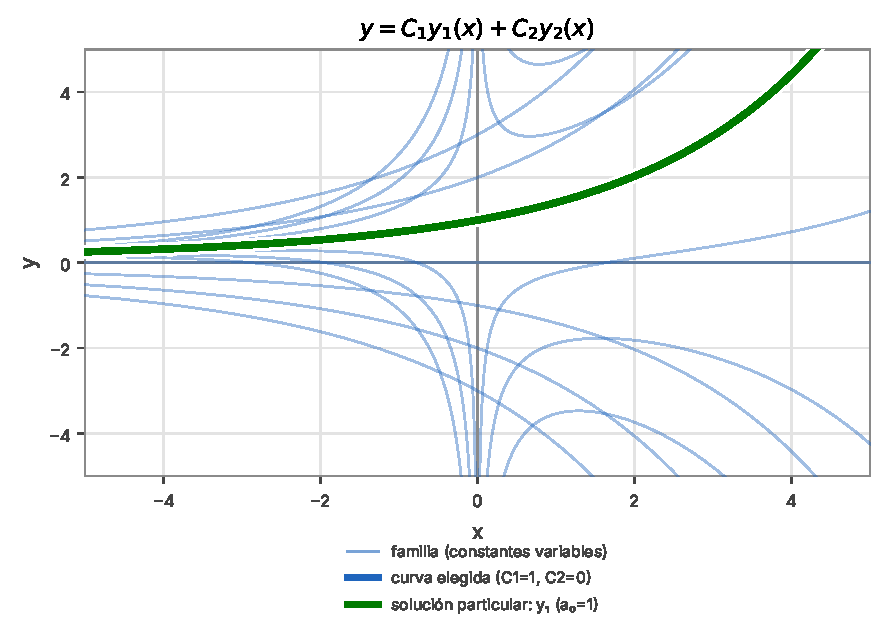
\includegraphics[width=0.8\linewidth]{h6-03-a.pdf}
\end{center}
\medskip
\noindent\textbf{(b) $\bm{2xy''+(x+1)y'+3y=0}$:} \\
$xP=\dfrac{x+1}{2}$ y $x^2Q=\dfrac{3x}{2}$ son analíticas $\implies$ $x=0$ es singular regular.

\vspace{0.2cm}\noindent\textbf{ $\bm{x>0}$.} Sustituyendo cada término ya desarrollado:
\begin{align*}
2xy'' &\to \sum_{n=0}^\infty 2(n+m)(n+m-1)a_nx^{n+m-1} \\
y' &\to \sum_{n=0}^\infty (n+m)a_nx^{n+m-1} \\
xy' &\to \sum_{n=0}^\infty (n+m)a_nx^{n+m} \\
3y &\to \sum_{n=0}^\infty 3a_nx^{n+m}
\end{align*}
Desplazamos $n\to n-1$ en los dos últimos:
\begin{align*}
xy' &\to \sum_{n=1}^\infty (n+m-1)a_{n-1}x^{n+m-1}, \qquad 3y \to \sum_{n=1}^\infty 3a_{n-1}x^{n+m-1}
\end{align*}

\[
\sum_{n=0}^\infty\Big[(n+m)\big(2(n+m)-1\big)a_n+(n+m+2)a_{n-1}\Big]x^{n+m-1}=0 \qquad (a_{-1}=0)
\]
$(n+m)\big(2(n+m)-1\big)a_n+(n+m+2)a_{n-1}=0$.\\
\smallskip\noindent Evaluada en $n=0$ : $m(2m-1)a_0=0$, y como $a_0\neq0$ queda la \emph{ecuación indicial} $m(2m-1)=0 \implies m_1=\tfrac12,\ m_2=0$.

\smallskip\noindent Evaluada en $n\geq1$ (recurrencia): $a_n=-\dfrac{(n+m+2)\,a_{n-1}}{(n+m)\big(2(n+m)-1\big)}$.

\smallskip\noindent $m=0$: $a_n=-\dfrac{(n+2)\,a_{n-1}}{n(2n-1)}$. evaluando:
\begin{align*}
a_1&=-\frac{3}{1\cdot1}a_0=-3a_0, & a_2&=-\frac{4}{2\cdot3}a_1=2a_0, \\
a_3&=-\frac{5}{3\cdot5}a_2=-\frac23a_0, & a_4&=-\frac{6}{4\cdot7}a_3=\frac17a_0.
\end{align*}

\smallskip\noindent $m=\tfrac12$: $a_n=-\dfrac{(2n+5)\,a_{n-1}}{2n\,(2n+1)}$. Desarrollando:
\begin{align*}
a_1&=-\frac{7}{2\cdot3}a_0=-\frac76a_0, & a_2&=-\frac{9}{4\cdot5}a_1=\frac{21}{40}a_0, \\
a_3&=-\frac{11}{6\cdot7}a_2=-\frac{11}{80}a_0, & a_4&=-\frac{13}{8\cdot9}a_3=\frac{143}{5760}a_0.
\end{align*}

\smallskip\noindent\textbf{Radio de convergencia.} Con $a_n=-\dfrac{(n+m+2)\,a_{n-1}}{(n+m)\big(2(n+m)-1\big)}$:
\[
\lim_{n\to\infty}\left|\frac{a_{n}x^{n}}{a_{n-1}x^{n-1}}\right|=\lim_{n\to\infty}\frac{(n+m+2)\,|x|}{(n+m)\big(2(n+m)-1\big)}=0<1 \quad\text{para todo }x,
\]
para $m=0$ y para $m=\tfrac12$. Luego $R=\infty$ en ambas series.

\vspace{0.2cm}\noindent\textbf{Caso $\bm{x<0}$.} Con $z=-x$: $(x+1)y'=(1-z)(-u')$, de modo que
\[
2zu''+(1-z)u'-3u=0
\]
Sustituyendo $u=\sum b_nz^{n+m}$ y desplazando $-zu'-3u$ ($n\to n-1$):
\[
\sum_{n=0}^\infty\Big[(n+m)\big(2(n+m)-1\big)b_n-(n+m+2)b_{n-1}\Big]z^{n+m-1}=0 \qquad (a_{-1}=0)
\]
La indicial es la misma y la recurrencia solo cambia el signo de $b_{n-1}$, luego $b_n=(-1)^na_n$. Como $z^n=(-x)^n$, al deshacer el cambio los coeficientes en $x$ son los mismos.
\[
\boxed{\begin{aligned}
y_1(x)&=a_0\left(1-3x+2x^2-\frac23x^3+\frac17x^4-\dots\right) \\[2pt]
y_2(x)&=a_0|x|^{1/2}\left(1-\frac76x+\frac{21}{40}x^2-\frac{11}{80}x^3+\dots\right)
\end{aligned}}
\]
\textit{Válidas para $x>0$ y para $x<0$ ($a_0$ es una constante arbitraria en cada una de las dos soluciones).}


\begin{center}
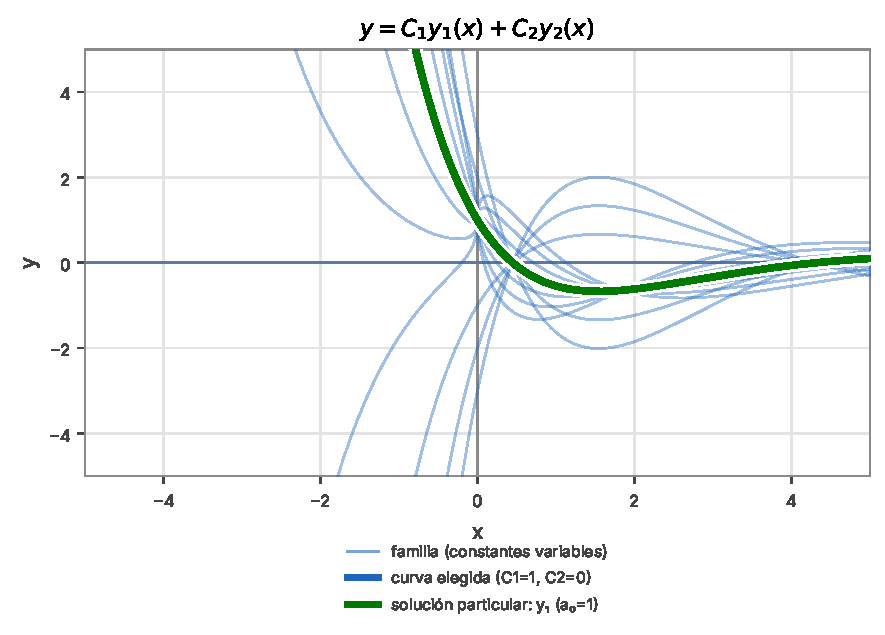
\includegraphics[width=0.8\linewidth]{h6-03-b.pdf}
\end{center}
\medskip
\noindent\textbf{(c) $\bm{2x^2y''+xy'-(x+1)y=0}$:} \\
$xP=\tfrac12$ y $x^2Q=-\dfrac{x+1}{2}$ son analíticas $\implies$ $x=0$ es singular regular.

\vspace{0.2cm}\noindent\textbf{Caso $\bm{x>0}$.}
\begin{align*}
2x^2y'' &\to \sum_{n=0}^\infty 2(n+m)(n+m-1)a_nx^{n+m} \\
xy' &\to \sum_{n=0}^\infty (n+m)a_nx^{n+m} \\
-xy &\to -\sum_{n=0}^\infty a_nx^{n+m+1} \;\xrightarrow{\,n\to n-1\,}\; -\sum_{n=1}^\infty a_{n-1}x^{n+m} \\
-y &\to -\sum_{n=0}^\infty a_nx^{n+m}
\end{align*}
\[
\sum_{n=0}^\infty\Big[\big(2(n+m)+1\big)(n+m-1)a_n-a_{n-1}\Big]x^{n+m}=0 \qquad (a_{-1}=0)
\]

\smallskip\noindent La relación de recurrencia va siendo $\big(2(n+m)+1\big)(n+m-1)a_n-a_{n-1}=0$.

\smallskip\noindent Evaluada en $n=0$, $(2m+1)(m-1)a_0=0$, la \emph{ecuación indicial} es $(2m+1)(m-1)=0 \implies m_1=1,\ m_2=-\tfrac12$.

 $a_n=\dfrac{a_{n-1}}{\big(2(n+m)+1\big)(n+m-1)}$.\\

\smallskip\noindent $m=1$: $a_n=\dfrac{a_{n-1}}{n(2n+3)}$. Desarrollando:
\[
a_1=\frac{a_0}{1\cdot5}=\frac{a_0}5,\quad a_2=\frac{a_1}{2\cdot7}=\frac{a_0}{70},\quad a_3=\frac{a_2}{3\cdot9}=\frac{a_0}{1890},\quad a_4=\frac{a_3}{4\cdot11}=\frac{a_0}{83160}
\]

\smallskip\noindent $m=-\tfrac12$: $a_n=\dfrac{a_{n-1}}{n(2n-3)}$. Desarrollando:
\[
a_1=\frac{a_0}{1\cdot(-1)}=-a_0,\quad a_2=\frac{a_1}{2\cdot1}=-\frac{a_0}2,\quad a_3=\frac{a_2}{3\cdot3}=-\frac{a_0}{18},\quad a_4=\frac{a_3}{4\cdot5}=-\frac{a_0}{360}
\]

\smallskip\noindent\textbf{Radio de convergencia.} Con $a_n=\dfrac{a_{n-1}}{\big(2(n+m)+1\big)(n+m-1)}$:
\[
\lim_{n\to\infty}\left|\frac{a_{n}x^{n}}{a_{n-1}x^{n-1}}\right|=\lim_{n\to\infty}\frac{|x|}{\big(2(n+m)+1\big)(n+m-1)}=0<1 \quad\text{para todo }x,
\]
para $m=1$ y para $m=-\tfrac12$. Luego $R=\infty$ en ambas series.

\vspace{0.2cm}\noindent\textbf{Caso $\bm{x<0}$.} Con $z=-x$ (nótese $xy'=zu'$ y $-(x+1)y=-(1-z)u$):
\[
2z^2u''+zu'-(1-z)u=0
\]
Sustituyendo $u=\sum b_nz^{n+m}$ y desplazando $zu$ ($n\to n-1$):
\[
\sum_{n=0}^\infty\Big[\big(2(n+m)+1\big)(n+m-1)b_n+b_{n-1}\Big]z^{n+m}=0 \qquad (a_{-1}=0)
\]
La indicial es la misma y la recurrencia equivale a $b_n=(-1)^na_n$.
\[
\boxed{\begin{aligned}
y_1(x)&=a_0|x|\left(1+\frac{x}{5}+\frac{x^2}{70}+\frac{x^3}{1890}+\dots\right) \\[2pt]
y_2(x)&=a_0|x|^{-1/2}\left(1-x-\frac{x^2}{2}-\frac{x^3}{18}-\frac{x^4}{360}-\dots\right)
\end{aligned}}
\]
\textit{Válidas para $x>0$ y para $x<0$ ($a_0$ es una constante arbitraria en cada una de las dos soluciones).}


\begin{center}
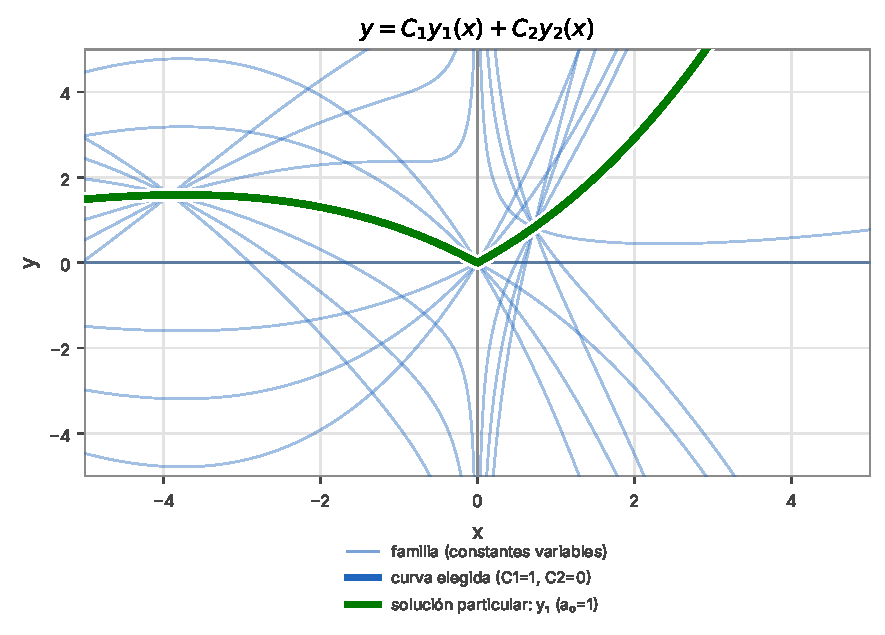
\includegraphics[width=0.8\linewidth]{h6-03-c.pdf}
\end{center}
\noindent\textbf{4. La EDO $\bm{4x^2y''-8x^2y'+(4x^2+1)y=0}$ tiene una sola solución en serie de Frobenius. Halladla.} \\
Dividiendo: $y''-2y'+\left(1+\dfrac{1}{4x^2}\right)y=0$, luego $xP=-2x$ y $x^2Q=x^2+\tfrac14$ son analíticas: $x=0$ es singular regular.

\vspace{0.2cm}\noindent\textbf{Caso $\bm{x>0}$.}
\begin{align*}
4x^2y'' &\to \sum_{n=0}^\infty 4(n+m)(n+m-1)a_nx^{n+m} \\
y &\to \sum_{n=0}^\infty a_nx^{n+m} \\
-8x^2y' &\to -\sum_{n=0}^\infty 8(n+m)a_nx^{n+m+1} \;\xrightarrow{\,n\to n-1\,}\; -\sum_{n=1}^\infty 8(n+m-1)a_{n-1}x^{n+m} \\
4x^2y &\to \sum_{n=0}^\infty 4a_nx^{n+m+2} \;\xrightarrow{\,n\to n-2\,}\; \sum_{n=2}^\infty 4a_{n-2}x^{n+m}
\end{align*}
\[
\sum_{n=0}^\infty\Big[\big(2(n+m)-1\big)^2a_n-8(n+m-1)a_{n-1}+4a_{n-2}\Big]x^{n+m}=0 \qquad (a_{-1}=a_{-2}=0)\\
\big(2(n+m)-1\big)^2a_n-8(n+m-1)a_{n-1}+4a_{n-2}=0 
\]

\smallskip\noindent $(2m-1)^2a_0=0 \implies (2m-1)^2=0 \implies m=\tfrac12$ (raíz doble, pues $a_0 \neq 0$).

\textit{Al ser la raíz doble, solo existe una solución de Frobenius (la otra contiene un término $\ln|x|$).} Con $m=\tfrac12$ la recurrencia (válida también para $n=1$ con $a_{-1}=0$) se simplifica a
\[
4n^2a_n=8\left(n-\tfrac12\right)a_{n-1}-4a_{n-2} \implies n^2a_n=(2n-1)a_{n-1}-a_{n-2}
\]

\begin{align*}
a_1&=a_0, & a_2&=\tfrac14\big(3a_1-a_0\big)=\tfrac12a_0, \\
a_3&=\tfrac19\big(5a_2-a_1\big)=\tfrac16a_0, & a_4&=\tfrac1{16}\big(7a_3-a_2\big)=\tfrac1{24}a_0
\end{align*}
Los valores sugieren $a_n=\dfrac{a_0}{n!}$. Por tanto $y=a_0 x^{1/2}\sum_{n=0}^\infty\dfrac{x^n}{n!}$ para $x>0$.

\smallskip\noindent\textbf{Radio de convergencia.} Para $a_n=\dfrac{a_0}{n!}$:
\[
\lim_{n\to\infty}\left|\frac{a_{n+1}x^{n+1}}{a_nx^n}\right|=\lim_{n\to\infty}\frac{|x|}{n+1}=0<1 \quad\text{para todo }x,
\]
luego $R=\infty$ (es la serie de $e^x$).

\vspace{0.2cm}\noindent\textbf{Caso $\bm{x<0}$.} Con $z=-x$ (ahora $-8x^2y'=-8z^2(-u')=+8z^2u'$):
\[
4z^2u''+8z^2u'+(4z^2+1)u=0
\]
Desplazando como antes, el único cambio es el signo del término en $b_{n-1}$: para $m=\tfrac12$,
\[
n^2b_n=-(2n-1)b_{n-1}-b_{n-2}
\]
cuya solución es $b_n=\dfrac{(-1)^n b_0}{n!}$. Entonces $u=b_0 z^{1/2}\sum_{n=0}^\infty \dfrac{(-z)^n}{n!}$ y, deshaciendo $z=-x$, $y=b_0(-x)^{1/2}\sum_{n=0}^\infty \dfrac{x^n}{n!}$.
\[
\boxed{y(x)= C |x|^{1/2}\sum_{n=0}^\infty\frac{x^n}{n!}}
\]
\textit{Válida para $x>0$ y para $x<0$, siendo $C$ una constante arbitraria.}\\


\begin{center}
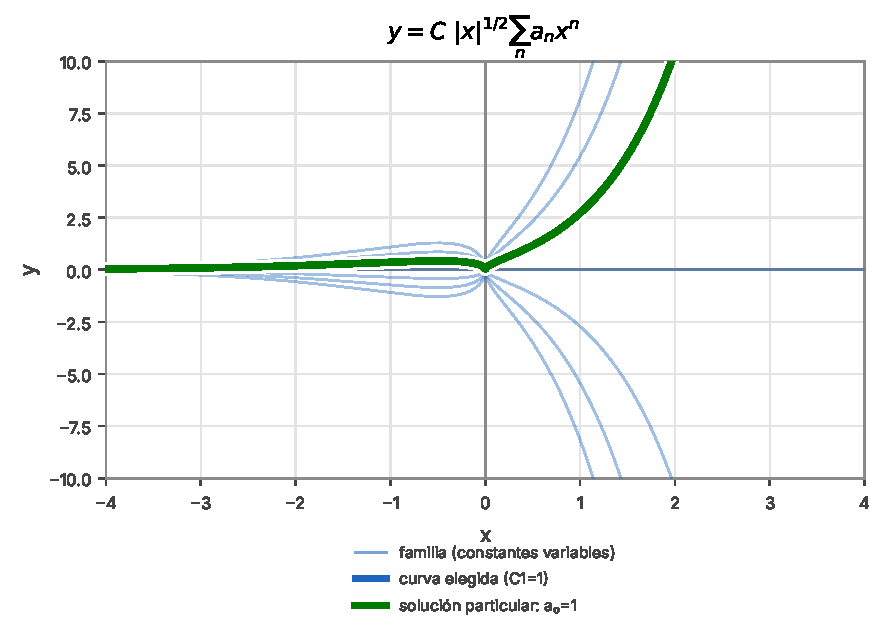
\includegraphics[width=0.8\linewidth]{h6-04.pdf}
\end{center}

\noindent\textbf{5. Hallad dos soluciones en serie de Frobenius independientes para cada una de las siguientes EDOs.}

\medskip
\noindent\textbf{(a) $\bm{x^2y''-x^2y'+(x^2-2)y=0}$:} \\
$xP=-x$ y $x^2Q=x^2-2$ analíticas $\implies$ $x=0$ es singular regular.

\vspace{0.2cm}\noindent\textbf{Caso $\bm{x>0}$.}
\begin{align*}
x^2y'' &\to \sum_{n=0}^\infty (n+m)(n+m-1)a_nx^{n+m} \\
-2y &\to -\sum_{n=0}^\infty 2a_nx^{n+m} \\
-x^2y' &\to -\sum_{n=0}^\infty (n+m)a_nx^{n+m+1} \;\xrightarrow{\,n\to n-1\,}\; -\sum_{n=1}^\infty (n+m-1)a_{n-1}x^{n+m} \\
x^2y &\to \sum_{n=0}^\infty a_nx^{n+m+2} \;\xrightarrow{\,n\to n-2\,}\; \sum_{n=2}^\infty a_{n-2}x^{n+m}
\end{align*}
\[
\sum_{n=0}^\infty\Big[(n+m-2)(n+m+1)a_n-(n+m-1)a_{n-1}+a_{n-2}\Big]x^{n+m}=0 \qquad (a_{-1}=a_{-2}=0)
\]

\smallskip\noindent $(n+m-2)(n+m+1)a_n-(n+m-1)a_{n-1}+a_{n-2}=0$.

\smallskip\noindent $n=0 \implies (m-2)(m+1)a_0=0 \implies (m-2)(m+1)=0 \implies m_1=2,\ m_2=-1$.

\smallskip\noindent Las raíces difieren en un entero ($3$), así que hay que comprobar que no aparece logaritmo.

\smallskip\noindent $m=2$: la recurrencia $n(n+3)a_n=(n+1)a_{n-1}-a_{n-2}$:
\begin{align*}
a_1&=\tfrac12a_0, & a_2&=\tfrac1{10}\Big(3a_1-a_0\Big)=\tfrac1{20}a_0, \\
a_3&=\tfrac1{18}\Big(4a_2-a_1\Big)=-\tfrac1{60}a_0, & a_4&=\tfrac1{28}\Big(5a_3-a_2\Big)=-\tfrac1{210}a_0, \\
a_5&=\tfrac1{40}\Big(6a_4-a_3\Big)=-\tfrac1{3360}a_0
\end{align*}

\smallskip\noindent $m=-1$: la recurrencia $n(n-3)a_n=(n-2)a_{n-1}-a_{n-2}$:
\begin{align*}
a_1&=\tfrac12a_0, & a_2&=-\tfrac12\Big(0\cdot a_1-a_0\Big)=\tfrac12a_0
\end{align*}
Para $n=3$: $0\cdot a_3=a_2-a_1=0$, que se cumple \emph{idénticamente}. Por tanto no aparece logaritmo y $a_3$ queda libre (elegirlo distinto de $0$ solo suma un múltiplo de $y_1$). Tomamos $a_3=0$ y seguimos:
\begin{align*}
a_4&=\tfrac14\Big(2a_3-a_2\Big)=-\tfrac18a_0, & a_5&=\tfrac1{10}\Big(3a_4-a_3\Big)=-\tfrac3{80}a_0, \\ a_6&=\tfrac1{18}\Big(4a_5-a_4\Big)=-\tfrac1{720}a_0
\end{align*}

\smallskip\noindent\textbf{Radio de convergencia.} La recurrencia tiene tres términos, así que no sirve el cociente de dos coeficientes. Aun así, de $(n+m-2)(n+m+1)a_n=(n+m-1)a_{n-1}-a_{n-2}$ se obtiene, para $n$ grande, $|a_n|\lesssim\dfrac{|a_{n-1}|}{n}+\dfrac{|a_{n-2}|}{n^2}$, es decir, $|a_n|$ decrece como $1/n!$ (los coeficientes calculados arriba lo muestran: $a_n/a_{n-1}\to0$) y $R=\infty$. Esto concuerda con el teorema de Frobenius: como $P=-1$ y $Q=1-\dfrac{2}{x^2}$ solo son singulares en $x=0$, la serie converge para todo $x\neq0$, es decir, $R=\infty$ en ambas series.

\vspace{0.2cm}\noindent\textbf{Caso $\bm{x<0}$.} Con $z=-x$ ($-x^2y'=+z^2u'$):
\[
z^2u''+z^2u'+(z^2-2)u=0
\]
\[
\sum_{n=0}^\infty\Big[(n+m-2)(n+m+1)b_n+(n+m-1)b_{n-1}+b_{n-2}\Big]z^{n+m}=0 \qquad (a_{-1}=a_{-2}=0)
\]
Misma indicial y recurrencia equivalente a $b_n=(-1)^na_n$ (de nuevo $0=0$ en $n=3$ para $m=-1$). Al deshacer el cambio:
\[
\boxed{\begin{aligned}y_1(x)&=a_0x^2\left(1+\frac{x}{2}+\frac{x^2}{20}-\frac{x^3}{60}-\frac{x^4}{210}-\frac{x^5}{3360}+\dots\right) \\[2pt] y_2(x)&=\frac{a_0}{|x|}\left(1+\frac{x}{2}+\frac{x^2}{2}-\frac{x^4}{8}-\frac{3x^5}{80}-\frac{x^6}{720}+\dots\right)\end{aligned}}
\]
\textit{Aquí $x^2=|x|^2$. Con $a_0$ constante arbitraria en cada solución.}


\begin{center}
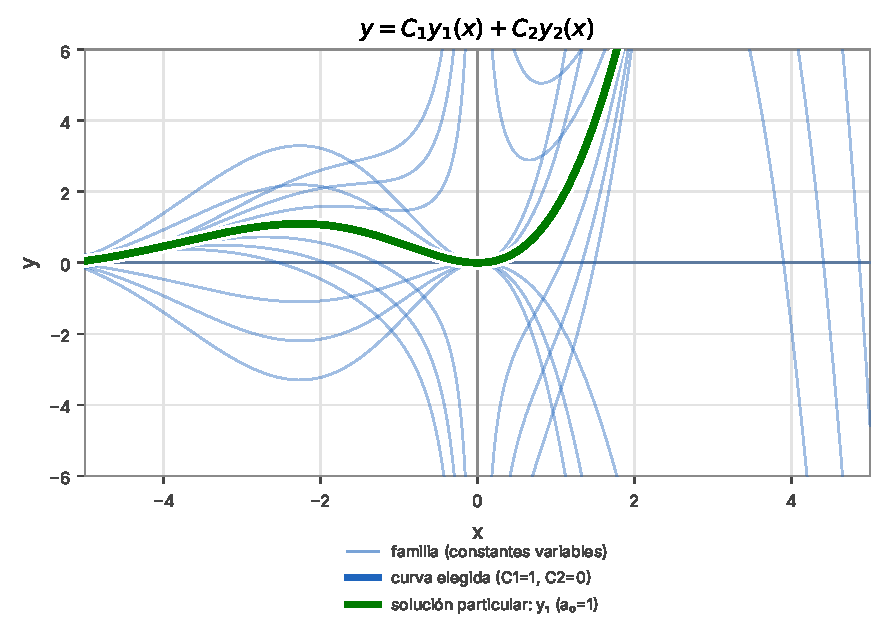
\includegraphics[width=0.8\linewidth]{h6-05-a.pdf}
\end{center}
\medskip
\noindent\textbf{(b) $\bm{xy''-y'+4x^3y=0}$:} \\
$P=-\dfrac1x$ y $Q=4x^2$: $xP=-1$ y $x^2Q=4x^4$ son analíticas $\implies$ $x=0$ es singular regular.

\vspace{0.2cm}\noindent\textbf{Caso $\bm{x>0}$.}
\begin{align*}
xy'' &\to \sum_{n=0}^\infty (n+m)(n+m-1)a_nx^{n+m-1} \\
-y' &\to -\sum_{n=0}^\infty (n+m)a_nx^{n+m-1} \\
4x^3y &\to \sum_{n=0}^\infty 4a_nx^{n+m+3} \;\xrightarrow{\,n\to n-4\,}\; \sum_{n=4}^\infty 4a_{n-4}x^{n+m-1}
\end{align*}
\[
\sum_{n=0}^\infty\Big[(n+m)(n+m-2)a_n+4a_{n-4}\Big]x^{n+m-1}=0 \qquad (a_{-1}=a_{-2}=a_{-3}=a_{-4}=0)
\]

\smallskip\noindent $(n+m)(n+m-2)a_n+4a_{n-4}=0$.

\smallskip\noindent $n=0 \implies m(m-2)a_0=0 \implies m(m-2)=0 \implies m_1=2,\ m_2=0$

\smallskip\noindent Evaluada en $n\geq1$ (recurrencia): $(n+m)(n+m-2)a_n=-4a_{n-4}$, donde $a_{n-4}=0$ si $n<4$.

\smallskip\noindent $m=2$: $n(n+2)a_n=0$ para $n=1,2,3$, luego $a_1=a_2=a_3=0$. Para $n\geq4$, $n(n+2)a_n=-4a_{n-4}$:
\[
a_4=-\frac{4}{4\cdot6}a_0=-\frac{a_0}{6},\quad a_8=-\frac{4}{8\cdot10}a_4=\frac{a_0}{120},\quad a_{12}=-\frac{4}{12\cdot14}a_8=-\frac{a_0}{5040}
\]
y los índices no múltiplos de $4$ son nulos. En general $a_{4k}=-\dfrac{4\,a_{4k-4}}{4k(4k+2)}=-\dfrac{a_{4k-4}}{2k(2k+1)}$, luego $a_{4k}=\dfrac{(-1)^k}{(2k+1)!}a_0$ y
\[
y_1=a_0\sum_{k=0}^\infty\frac{(-1)^k}{(2k+1)!}x^{4k+2}
\]

\smallskip\noindent $m=0$: $n(n-2)a_n=0$ para $n=1,2,3$. Para $n=1$ y $n=3$: $a_1=a_3=0$. Para $n=2$ la ecuación es $0\cdot a_2=0$, que se cumple (sin logaritmo); $a_2$ queda libre y lo tomamos nulo (si no, solo suma un múltiplo de $y_1$). Para $n\geq4$, $n(n-2)a_n=-4a_{n-4}$:
\[
a_4=-\frac{4}{4\cdot2}a_0=-\frac{a_0}{2},\quad a_8=-\frac{4}{8\cdot6}a_4=\frac{a_0}{24},\quad a_{12}=-\frac{4}{12\cdot10}a_8=-\frac{a_0}{720}
\]
En general $a_{4k}=-\dfrac{4\,a_{4k-4}}{4k(4k-2)}=-\dfrac{a_{4k-4}}{2k(2k-1)}$, luego $a_{4k}=\dfrac{(-1)^k}{(2k)!}a_0$ y
\[
y_2=a_0\sum_{k=0}^\infty\frac{(-1)^k}{(2k)!}x^{4k}
\]

\smallskip\noindent\textbf{Radio de convergencia.} Solo hay potencias de $x$ separadas de cuatro en cuatro, así que se aplica el cociente entre términos consecutivos no nulos ($n\to n+4$), usando $(n+m)(n+m-2)a_n=-4a_{n-4}$:
\[
\lim_{n\to\infty}\left|\frac{a_{n+4}x^{n+4}}{a_nx^n}\right|=\lim_{n\to\infty}\frac{4\,|x|^4}{(n+4+m)(n+2+m)}=0<1 \quad\text{para todo }x,
\]
para $m=2$ y para $m=0$. Luego $R=\infty$ en ambas series.

\vspace{0.2cm}\noindent\textbf{Caso $\bm{x<0}$.} Con $z=-x$: $xy''=-zu''$, $-y'=u'$ y $4x^3y=-4z^3u$, de modo que
\[
-zu''+u'-4z^3u=0 \iff zu''-u'+4z^3u=0
\]
que es \emph{la misma EDO} en $z>0$. Por tanto, las soluciones son las mismas.
\[
\boxed{\begin{aligned}y_1(x)&=a_0\sum_{k=0}^\infty\frac{(-1)^k}{(2k+1)!}x^{4k+2} \\[2pt] y_2(x)&=a_0\sum_{k=0}^\infty\frac{(-1)^k}{(2k)!}x^{4k}\end{aligned}}
\]
\textit{Válidas para $x>0$ y para $x<0$; $a_0$ arbitraria en cada solución.}


\begin{center}
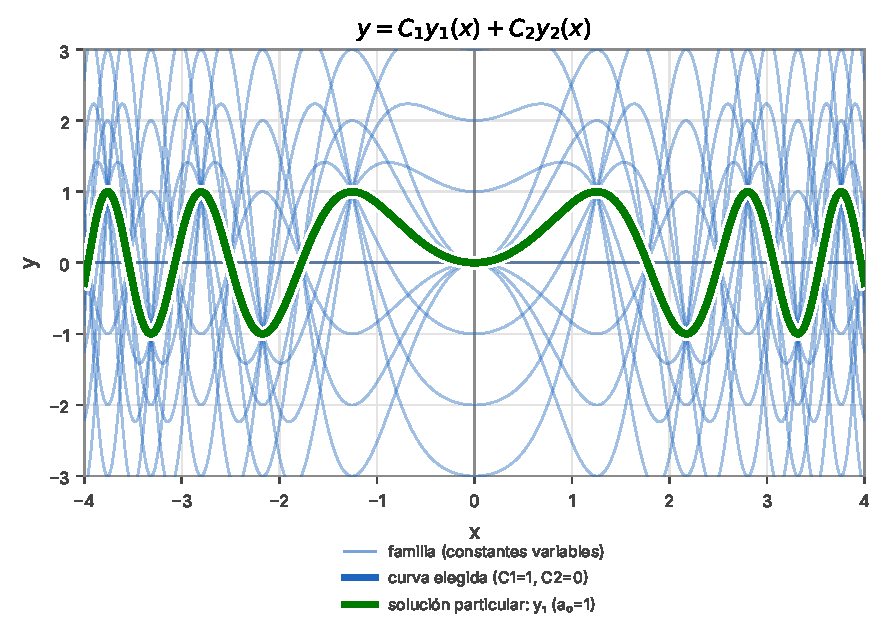
\includegraphics[width=0.8\linewidth]{h6-05-b.pdf}
\end{center}
\medskip
\noindent\textbf{(c) $\bm{2x^2y''+(3x-x^2)y'-(x+1)y=0}$:} \\
$xP=\dfrac{3-x}{2}$ y $x^2Q=-\dfrac{x+1}{2}$ analíticas $\implies$ $x=0$ es singular regular.

\vspace{0.2cm}\noindent\textbf{Caso $\bm{x>0}$.}
\begin{align*}
2x^2y'' &\to \sum_{n=0}^\infty 2(n+m)(n+m-1)a_nx^{n+m} \\
3xy' &\to \sum_{n=0}^\infty 3(n+m)a_nx^{n+m} \\
-y &\to -\sum_{n=0}^\infty a_nx^{n+m} \\
-x^2y' &\to -\sum_{n=0}^\infty (n+m)a_nx^{n+m+1} \;\xrightarrow{\,n\to n-1\,}\; -\sum_{n=1}^\infty (n+m-1)a_{n-1}x^{n+m} \\
-xy &\to -\sum_{n=0}^\infty a_nx^{n+m+1} \;\xrightarrow{\,n\to n-1\,}\; -\sum_{n=1}^\infty a_{n-1}x^{n+m}
\end{align*}
\[
\sum_{n=0}^\infty\Big[\big(2(n+m)-1\big)(n+m+1)a_n-(n+m)a_{n-1}\Big]x^{n+m}=0 \qquad (a_{-1}=0)
\]

\smallskip\noindent $\big(2(n+m)-1\big)(n+m+1)a_n-(n+m)a_{n-1}=0$.

\smallskip\noindent $(2m-1)(m+1)a_0=0 \implies (2m-1)(m+1)=0 \implies m_1=\tfrac12,\ m_2=-1$.

\

\smallskip\noindent $m=\tfrac12$: $n(2n+3)a_n=\dfrac{2n+1}{2}a_{n-1}$. Desarrollando:
\[
\begin{aligned}a_1&=\frac{3/2}{1\cdot5}a_0=\frac3{10}a_0, & a_2&=\frac{5/2}{2\cdot7}a_1=\frac3{56}a_0, \\ a_3&=\frac{7/2}{3\cdot9}a_2=\frac1{144}a_0, & a_4&=\frac{9/2}{4\cdot11}a_3=\frac{1}{1408}a_0\end{aligned}
\]

\smallskip\noindent $m=-1$: $n(2n-3)a_n=(n-1)a_{n-1}$. Para $n=1$: $-a_1=0\implies a_1=0$, y por recurrencia $a_n=0$ para todo $n\geq1$. La serie se reduce a un solo término.

\smallskip\noindent\textbf{Radio de convergencia.} Para $m=\tfrac12$, de $n(2n+3)a_n=\dfrac{2n+1}{2}a_{n-1}$:
\[
\lim_{n\to\infty}\left|\frac{a_{n}x^{n}}{a_{n-1}x^{n-1}}\right|=\lim_{n\to\infty}\frac{(2n+1)\,|x|}{2n(2n+3)}=0<1 \quad\text{para todo }x,
\]
luego $R=\infty$. Para $m=-1$ la serie tiene un solo término ($y_2=a_0/x$), así que no hay nada que comprobar.

\vspace{0.2cm}\noindent\textbf{Caso $\bm{x<0}$.} Con $z=-x$: $(3x-x^2)y'=(-3z-z^2)(-u')=(3z+z^2)u'$ y $-(x+1)y=-(1-z)u$:
\[
2z^2u''+(3z+z^2)u'-(1-z)u=0
\]
Desplazando $z^2u'$ y $zu$ ($n\to n-1$):
\[
\sum_{n=0}^\infty\Big[\big(2(n+m)-1\big)(n+m+1)b_n+(n+m)b_{n-1}\Big]z^{n+m}=0 \qquad (a_{-1}=0)
\]
L recurrencia equivale a $b_n=(-1)^na_n$. Para $m=-1$ de nuevo $b_1=0$ y $u_2=z^{-1}$, es decir, $y_2=-\dfrac1x$, que es múltiplo de $1/x$.

\textit{Comprobación con $y_2=1/x$: $2x^2\cdot\frac{2}{x^3}+(3x-x^2)\left(-\frac1{x^2}\right)-\frac{x+1}{x}=\frac4x-\frac3x+1-1-\frac1x=0$ \checkmark (para todo $x\neq0$).}
\[
\boxed{\begin{aligned}y_1(x)&=a_0|x|^{1/2}\left(1+\frac{3x}{10}+\frac{3x^2}{56}+\frac{x^3}{144}+\dots\right) \\[2pt] y_2(x)&=\frac{a_0}{x}\end{aligned}} \qquad \text{\textit{($a_0$ arbitraria en cada solución)}}
\]



\begin{center}
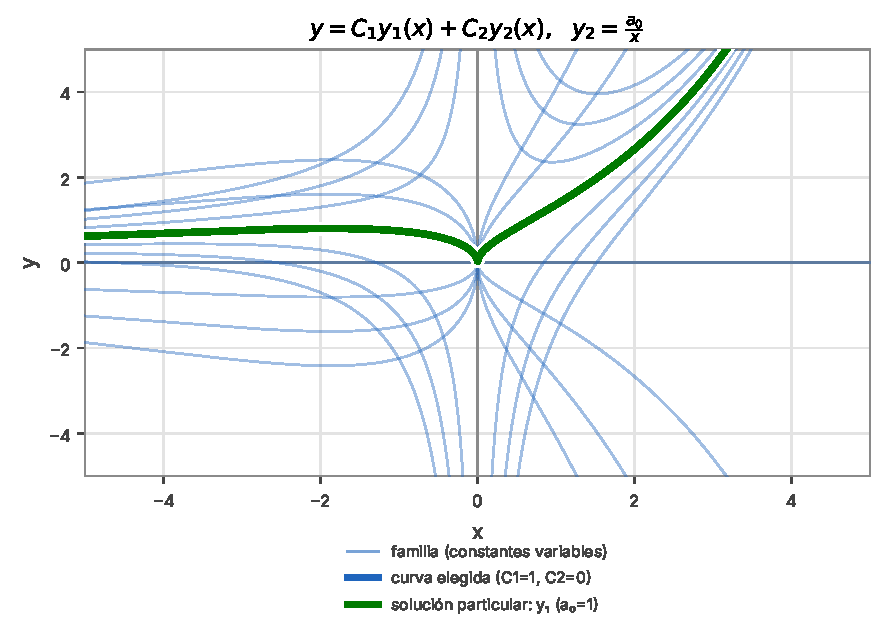
\includegraphics[width=0.8\linewidth]{h6-05-c.pdf}
\end{center}
\noindent\textbf{6. La ecuación de Bessel de orden $\bm{p=1}$ es $\bm{x^2y''+xy'+(x^2-1)y=0}$. Demostrad que $\bm{m_1-m_2=2}$, que la ecuación solo tiene una solución en forma de serie de Frobenius y halladla.} \\
$xP=1$ y $x^2Q=x^2-1$ son analíticas $\implies$ $x=0$ es singular regular.

\vspace{0.2cm}\noindent\textbf{Caso $\bm{x>0}$.}
\begin{align*}
x^2y'' &\to \sum_{n=0}^\infty (n+m)(n+m-1)a_nx^{n+m} \\
xy' &\to \sum_{n=0}^\infty (n+m)a_nx^{n+m} \\
-y &\to -\sum_{n=0}^\infty a_nx^{n+m} \\
x^2y &\to \sum_{n=0}^\infty a_nx^{n+m+2} \;\xrightarrow{\,n\to n-2\,}\; \sum_{n=2}^\infty a_{n-2}x^{n+m}
\end{align*}
\[
\sum_{n=0}^\infty\Big[\big((n+m)^2-1\big)a_n+a_{n-2}\Big]x^{n+m}=0 \qquad (a_{-1}=a_{-2}=0)
\]

\smallskip\noindent $\big((n+m)^2-1\big)a_n+a_{n-2}=0$.

\smallskip\noindent $m^2-1=0 \implies m_1=1,\ m_2=-1 \implies m_1-m_2=2 \quad\blacksquare$.


\smallskip\noindent $m=m_2=-1$: $n=1$ da $-a_1=0\implies a_1=0$. Para $n=2$: $0\cdot a_2=-a_0\implies a_0=0$, \emph{contradicción} con $a_0\neq0$. Luego \textbf{no existe} solución de Frobenius con $m_2=-1$ (la segunda solución lleva un término $\ln|x|$).

\smallskip\noindent $m=m_1=1$: $n=1$ da $3a_1=0\implies a_1=0$ y por la recurrencia todos los impares son nulos. Para $n\geq2$: $n(n+2)a_n=-a_{n-2}$, luego
\[
a_2=-\frac{a_0}{2\cdot4}=-\frac{a_0}{8},\quad a_4=-\frac{a_2}{4\cdot6}=\frac{a_0}{192},\quad a_6=-\frac{a_4}{6\cdot8}=-\frac{a_0}{9216}
\]

\smallskip\noindent\textbf{Radio de convergencia.} Para $m=1$, de $n(n+2)a_n=-a_{n-2}$ (solo hay potencias pares, $n\to n+2$):
\[
\lim_{n\to\infty}\left|\frac{a_{n+2}x^{n+2}}{a_nx^n}\right|=\lim_{n\to\infty}\frac{|x|^2}{(n+2)(n+4)}=0<1 \quad\text{para todo }x,
\]
luego $R=\infty$. (Para $m=-1$ no existe serie de Frobenius, así que no hay nada que comprobar.)

\vspace{0.2cm}\noindent\textbf{Caso $\bm{x<0}$.} Con $z=-x$ (como $x^2y''=z^2u''$, $xy'=(-z)(-u')=zu'$ y $x^2=z^2$):
\[
z^2u''+zu'+(z^2-1)u=0
\]
que es \emph{la misma ecuación} en $z>0$. Así la indicial y la recurrencia son idénticas.\\

\[
\boxed{y_1(x)=a_0\left(x-\frac{x^3}{8}+\frac{x^5}{192}-\dots\right) \;}
\]
\textit{Válida para $x>0$ y para $x<0$.}


\begin{center}
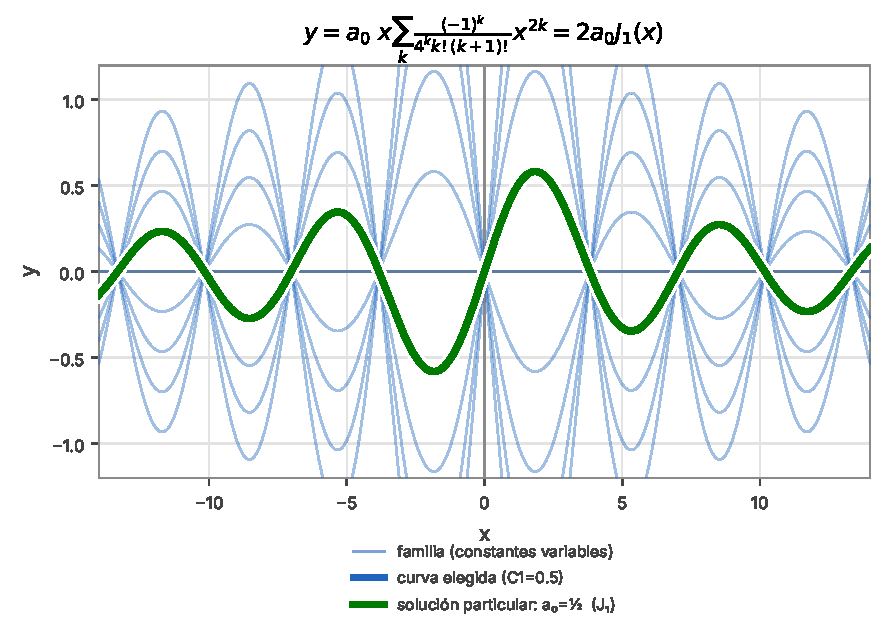
\includegraphics[width=0.8\linewidth]{h6-06.pdf}
\end{center}

\noindent\textbf{7. Hallad una solución en forma de serie de Frobenius en $\bm{x}$ de $y''+k\left(E-\dfrac{Ae^{-\alpha x}}{x}\right)y=0$ (basta con tres términos).} \\
Aquí $P=0$ y $Q=k\left(E-\dfrac{Ae^{-\alpha x}}{x}\right)$, luego $xP=0$ y $x^2Q=kEx^2-kAxe^{-\alpha x}$, ambas analíticas $\implies$ $x=0$ es singular regular.

\vspace{0.2cm}\noindent\textbf{Caso $\bm{x>0}$.} Proponemos $y=\sum_{n=0}^\infty a_nx^{n+m}$ con $a_0\neq0$. La exponencial se desarrolla como serie de potencias,
\[
e^{-\alpha x}=\sum_{j=0}^\infty c_jx^j, \qquad c_j=\frac{(-\alpha)^j}{j!},
\]
y el producto del coeficiente de $x^{n+m}$ en $e^{-\alpha x}y$ es $\sum_{j=0}^{n}c_j\,a_{n-j}$, es decir,
\[
e^{-\alpha x}\,y=\sum_{n=0}^\infty\left[\sum_{j=0}^{n}\frac{(-\alpha)^j}{j!}\,a_{n-j}\right]x^{n+m}
\]
Sustituyendo cada término, sin multiplicar la ecuación por nada:
\begin{align*}
y'' &\to \sum_{n=0}^\infty (n+m)(n+m-1)a_nx^{n+m-2} \\
kEy &\to \sum_{n=0}^\infty kE\,a_nx^{n+m} \;\xrightarrow{\,n\to n-2\,}\; \sum_{n=2}^\infty kE\,a_{n-2}x^{n+m-2} \\
-\frac{kAe^{-\alpha x}}{x}\,y &\to -kA\sum_{n=0}^\infty\left[\sum_{j=0}^{n}\frac{(-\alpha)^j}{j!}\,a_{n-j}\right]x^{n+m-1} \\
&\xrightarrow{\,n\to n-1\,}\; -kA\sum_{n=1}^\infty\left[\sum_{j=0}^{n-1}\frac{(-\alpha)^j}{j!}\,a_{n-1-j}\right]x^{n+m-2}
\end{align*}
\[
\sum_{n=0}^\infty\Bigg[(n+m)(n+m-1)a_n+kE\,a_{n-2}-kA\sum_{j=0}^{n-1}\frac{(-\alpha)^j}{j!}\,a_{n-1-j}\Bigg]x^{n+m-2}=0
\]

\[
(n+m)(n+m-1)\,a_n+kE\,a_{n-2}-kA\sum_{j=0}^{n-1}\frac{(-\alpha)^j}{j!}\,a_{n-1-j}=0
\]

\smallskip\noindent Evaluada en $n=0$ (la suma se vacía y $a_{-2}=0$): $m(m-1)a_0=0$, y como $a_0\neq0$ queda  $m(m-1)=0 \implies m_1=1,\ m_2=0$.

\smallskip\noindent Tomamos la raíz mayor $m=1$. Para $n\geq1$ la recurrencia general queda
\[
a_n=\frac{1}{n(n+1)}\left[kA\sum_{j=0}^{n-1}\frac{(-\alpha)^j}{j!}\,a_{n-1-j}-kE\,a_{n-2}\right]
\]

\smallskip\noindent\ Para $n=1,2,3$. La suma de vale $S_0=a_0$, $S_1=a_1-\alpha a_0$ y $S_2=a_2-\alpha a_1+\tfrac{\alpha^2}{2}a_0$:
\begin{align*}
n=1&: \quad 2a_1=kA\,a_0 \implies a_1=\frac{kA}{2}a_0 \\
n=2&: \quad 6a_2=kA(a_1-\alpha a_0)-kE\,a_0 \implies a_2=\frac{k\left(kA^2-2\alpha A-2E\right)}{12}a_0 \\
n=3&: \quad 12a_3=kA\left(a_2-\alpha a_1+\tfrac{\alpha^2}{2}a_0\right)-kE\,a_1 \implies a_3=\frac{kA\left(k^2A^2-8\alpha kA-8kE+6\alpha^2\right)}{144}a_0
\end{align*}

\vspace{0.2cm}\noindent\textbf{Caso $\bm{x<0}$.} Con $z=-x>0$, $y(x)=u(z)$ ($y''=u''$) y $e^{-\alpha x}=e^{\alpha z}$: $-\dfrac{kAe^{-\alpha x}}{x}y=+\dfrac{kAe^{\alpha z}}{z}u$, de modo que
\[
u''+k\left(E+\frac{Ae^{\alpha z}}{z}\right)u=0
\]
que es la ecuación anterior con $A\to-A$ y $\alpha\to-\alpha$. Repitiendo para $u=\sum b_nz^{n+m}$ y $m=1$:
\[
n(n+1)\,b_n=-kA\sum_{j=0}^{n-1}\frac{\alpha^j}{j!}\,b_{n-1-j}-kE\,b_{n-2}
\]
que es la recurrencia de $a_n$ multiplicada por $(-1)^n$. En particular
\[
b_1=-\frac{kA}{2}b_0,\qquad b_2=\frac{k\left(kA^2-2\alpha A-2E\right)}{12}b_0,\qquad b_3=-\frac{kA\left(k^2A^2-8\alpha kA-8kE+6\alpha^2\right)}{144}b_0
\]
Como $z^n=(-x)^n$, al volver a $x$ los coeficientes de $x^n$ son los mismos: $y=-b_0\,x\,[1+\dots]=b_0\,|x|\,[1+\dots]$ con la misma serie.
\[
\boxed{\begin{aligned}y(x)=a_0\,|x|\Big[&1+\frac{kA}{2}\,x+\frac{k\left(kA^2-2\alpha A-2E\right)}{12}\,x^2 \\ &+\frac{kA\left(k^2A^2-8\alpha kA-8kE+6\alpha^2\right)}{144}\,x^3+\dots\Big]\end{aligned}}
\]


\begin{center}
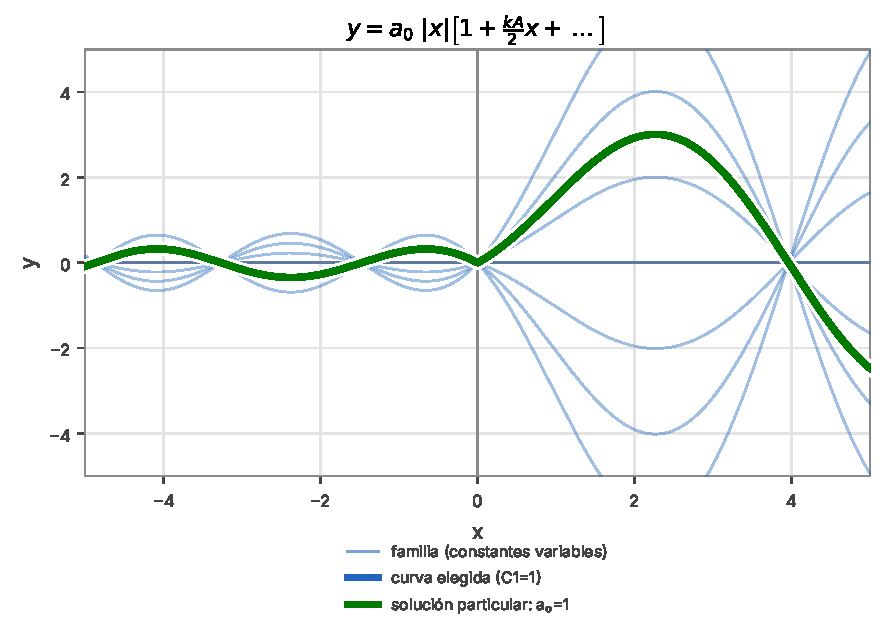
\includegraphics[width=0.8\linewidth]{h6-07.pdf}
\end{center}

\end{document}
